\section{Odolnost proti násilnému vniknutí}
Základní druhý namáhání, kterým musí trezor odolat, jsou

\begin{itemize}
    \item snaha o vytržení dveří 
    \item snaha o odemčení bez znalosti hesla
\end{itemize}

\paragraph{Vytržení dveří}
Jedním ze způsobů~namáhání~mechanizmu~je~vytržení~dveří~z~trezoru.

\subsection{Západka}

\begin{figure}[htbp]
    \centering
    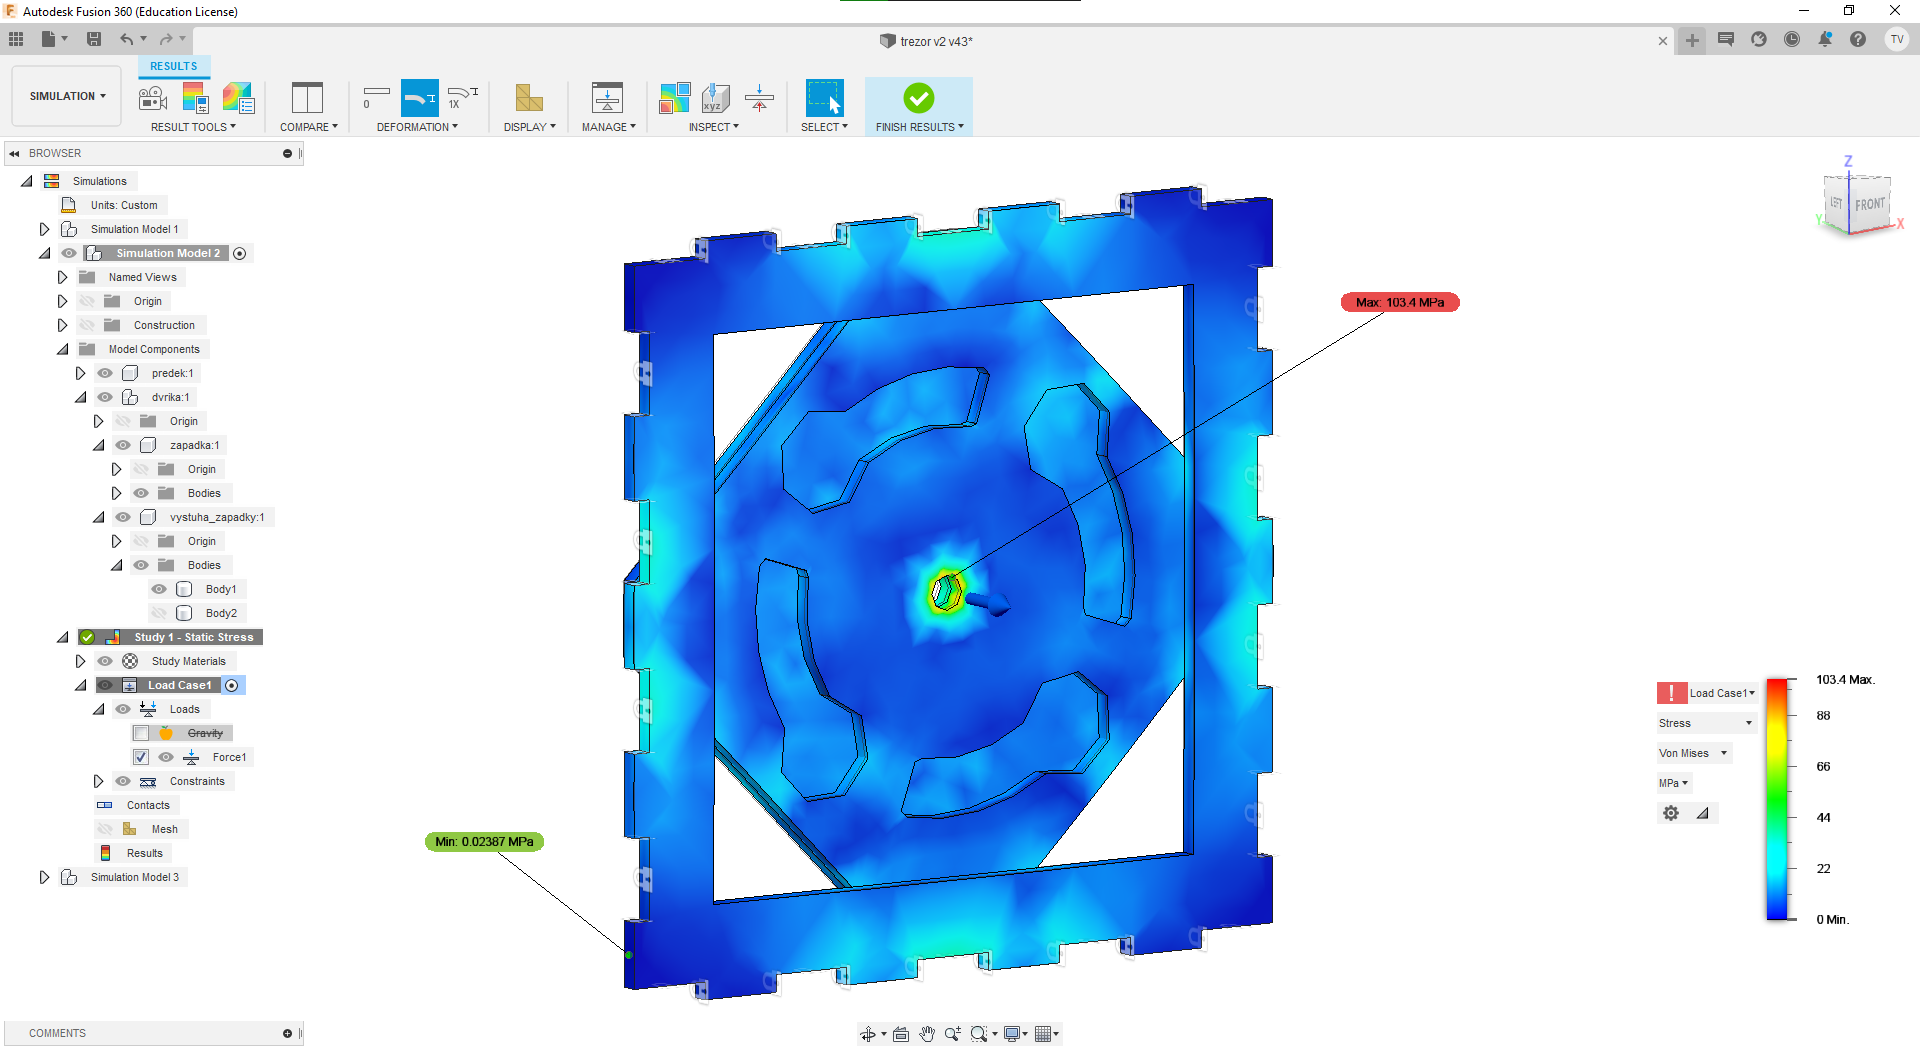
\includegraphics[width=\textwidth]{kapitoly/obrazky/M3/simulace/odolnost_proti_vytrzeni_4kN.png}
    \caption{simulace pokusu o vytržení dveří silou 4 000 N}
    \label{fig:M3-simulace-vytrzeni}
\end{figure}
Ke kompletní simulaci se můžete dostat \href{https://myhub.autodesk360.com/ue2d7aa41/g/shares/SH56a43QTfd62c1cd96843f1e03a0eb48053?viewState=NoIgbgDAdAjCA0IDeAdEAXAngBwKZoC40BlASwFsBXAGwEN1SB7AOzXjVoGdPd1C0ARjABsATlEQItALQBjcbmkAWCMIjSBuWgA5lAM22ilAVgAmMAOyy9\%2BBGkYCAVrlnoAkqcIBmAL4gAukA}{zde}
po kliknutí na \uv{Simulation} a~\uv{Simulation Model 2}. V tabulce napravo se pak můžete přepínat mezi barevným zobrazení několika veličin.

\newpage

\subsection{Kolík}
Při pokusu o vytržení je celá síla přenášena kolíkem.

 $ \sigma_{max} = 132  $ MPa    ( \href{https://is.mendelu.cz/eknihovna/opory/zobraz_cast.pl?fit_w=1;cast=9190}{dubové dřevo ve směru vláken při vlhkosti 12 \% }) % strana 22 tabulka 2 -> https://www.vutbr.cz/www_base/zav_prace_soubor_verejne.php?file_id=66237

$D = 6 mm$ %todo popis všech veličin

 \(\sigma_{max} = F/S \Rightarrow F = \sigma_{max} \cdot S = 132 \cdot (\pi \cdot D^2/4) = 3 732,21 N \)  z toho a ze simulace vyplývá že kolík je při namáhání nejslabším členem, přesto že ne o moc.

\paragraph{Otevření bez odemčení}
Dalším způsobem namáhání může být snaha otočit západkou pez zadání správného hesla.

\subparagraph{Západka}

\begin{figure}[htbp]
    \centering
    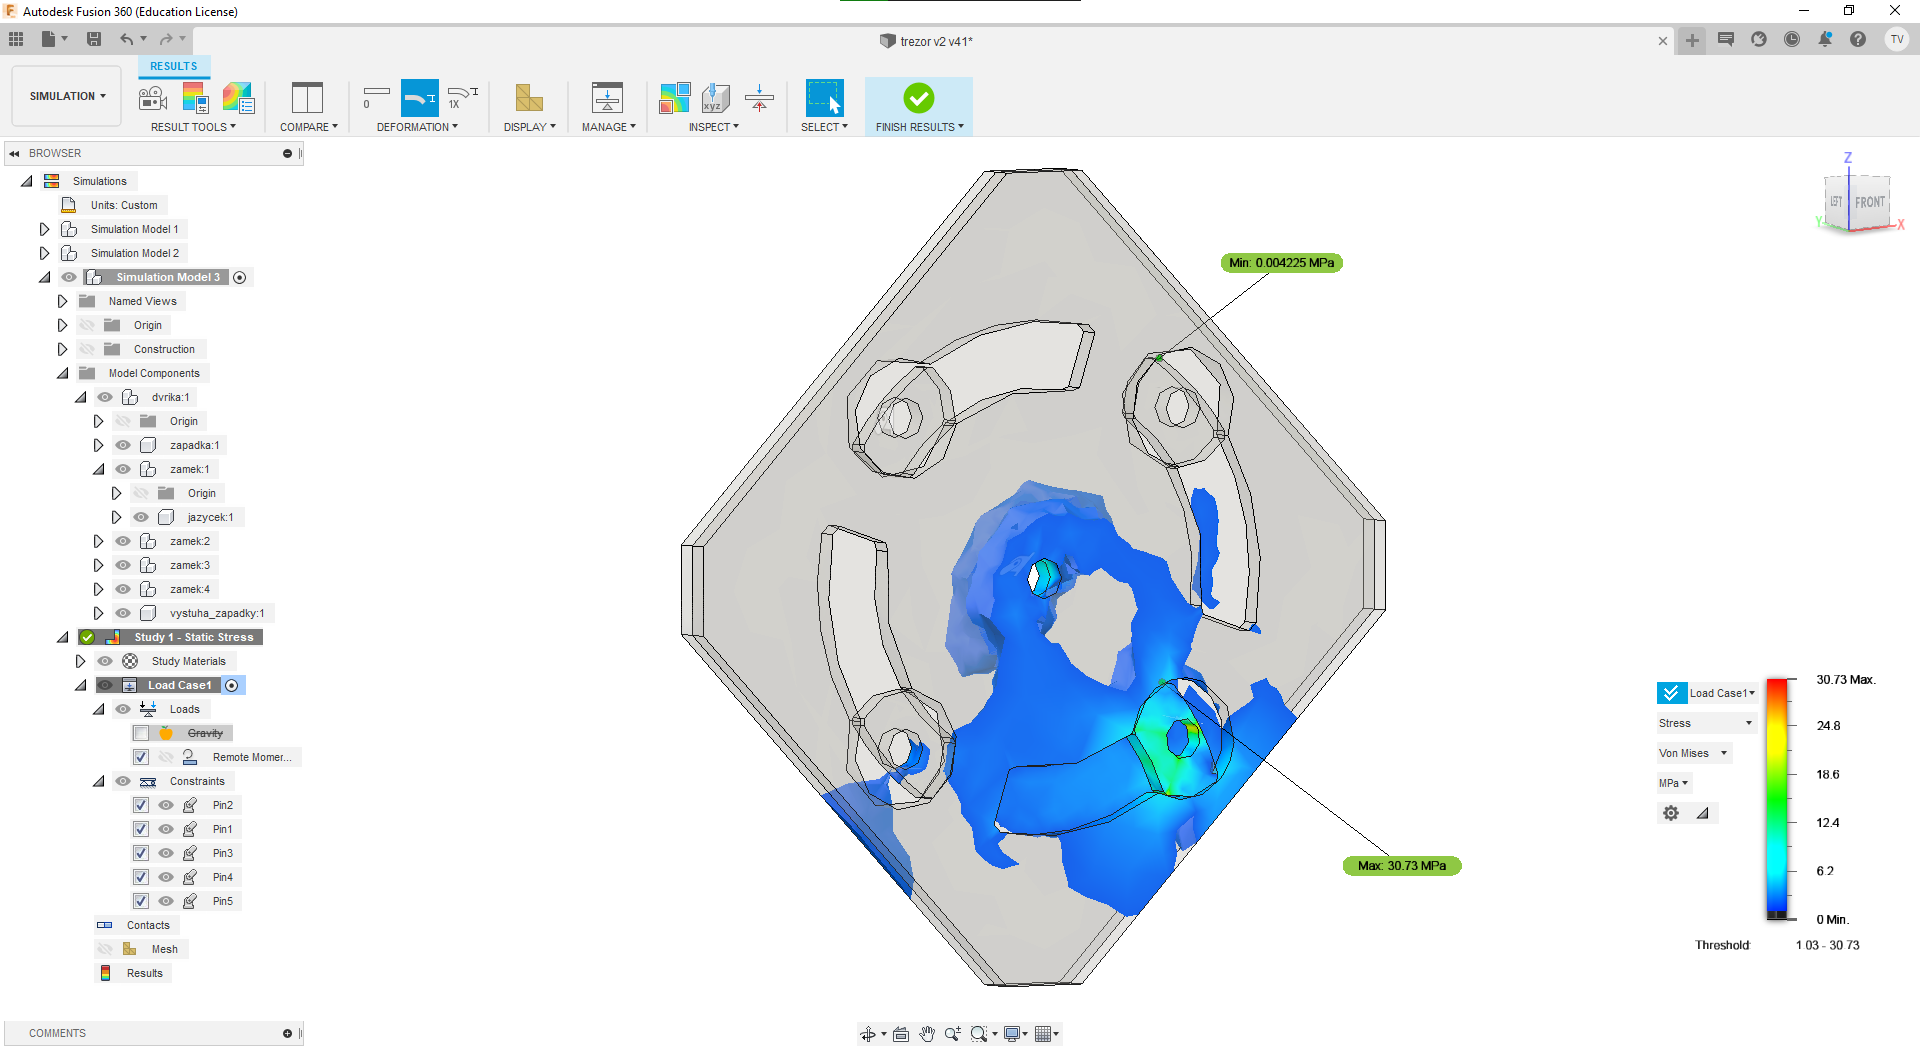
\includegraphics[width=\textwidth]{kapitoly/obrazky/M3/simulace/odolnost_proti_nasilnemu_odemceni_10Nm.png}
    \caption{simulace pokusu o otevření bez předchozího odemčení při kroutícím momentu 10 000 Nmm, zobrazeno jen napětí nad 1 MPa}
    \label{fig:M3-simulace-vytrzeni}
\end{figure}

Ke kompletní simulaci se můžete dostat \href{https://myhub.autodesk360.com/ue2d7aa41/g/shares/SH56a43QTfd62c1cd96843f1e03a0eb48053?viewState=NoIgbgDAdAjCA0IDeAdEAXAngBwKZoC40BlASwFsBXAGwEN1SB7AOzXjVoGdPd1C0ARjABsATlEQItALQBjcbmkAWCMIjSBuWgA5lAM22ilAVgAmMAOyy9\%2BBGkYCAVrlnoAkqcIBmAL4gAukA}{zde}
po kliknutí na \uv{Simulation} a~\uv{Simulation Model 3}. V tabulce napravo se pak můžete přepínat mezi barevným zobrazení několika veličin.

\subparagraph{Kolík}
Kroutící moment, který je dřevěný kolík o průměru D = 6~mm schopen přenést. 

\(\tau_{max} = 52,3\) MPa (\href{https://is.mendelu.cz/eknihovna/opory/zobraz_cast.pl?fit_w=1;cast=9190}{dubové dřevo ve směru vláken při vlhkosti 12 \% })

$ \tau_{max} = \frac{M_k}{W_k} \Rightarrow M_k = \tau_{max} \cdot W_k = \sigma _d \cdot \frac{\pi \cdot D^3}{16} $ %todo popis všech veličin

\(M_k = 52,3 \cdot \frac{\pi \cdot 6^3}{16} = 2 218,16\) N*mm. Z výpočtu a ze simulace plyne, že kolík je při namáhání v krutu nejslabším místem. Pro zvýšení odolnosti by proto bylo 
potřeba zvětšit kolík nebo změnit materiál.